\documentclass{beamer}
\beamertemplatenavigationsymbolsempty
\usecolortheme{beaver}
\setbeamertemplate{blocks}[rounded=true, shadow=true]
\setbeamertemplate{footline}[page number]

%
\usepackage[utf8]{inputenc}
\usepackage[english,russian]{babel}
\usepackage{amssymb,amsfonts,amsmath,mathtext}
\usepackage[]{algorithmic}
\usepackage{subfig}
\usepackage[all]{xy} % xy package for diagrams
\usepackage{array}
\usepackage{tikz}
\usepackage{multicol}% many columns in slide
\usepackage{hyperref}% urls
\usepackage{hhline}%tables
% Your figures are here:
\graphicspath{ {fig/} {../fig/} }

\usepackage{tikz}
\usetikzlibrary{shapes,arrows}



\newcommand{\bz}{\mathbf{z}}
\newcommand{\bx}{\mathbf{x}}
\newcommand{\by}{\mathbf{y}}
\newcommand{\bv}{\mathbf{v}}
\newcommand{\bw}{\mathbf{w}}
\newcommand{\ba}{\mathbf{a}}
\newcommand{\bb}{\mathbf{b}}
\newcommand{\bp}{\mathbf{p}}
\newcommand{\bq}{\mathbf{q}}
\newcommand{\bt}{\mathbf{t}}
\newcommand{\bu}{\mathbf{u}}
\newcommand{\bT}{\mathbf{T}}
\newcommand{\bX}{\mathbf{X}}
\newcommand{\bZ}{\mathbf{Z}}
\newcommand{\bS}{\mathbf{S}}
\newcommand{\bH}{\mathbf{H}}
\newcommand{\bW}{\mathbf{W}}
\newcommand{\bY}{\mathbf{Y}}
\newcommand{\bU}{\mathbf{U}}
\newcommand{\bQ}{\mathbf{Q}}
\newcommand{\bP}{\mathbf{P}}
\newcommand{\bA}{\mathbf{A}}
\newcommand{\bB}{\mathbf{B}}
\newcommand{\bC}{\mathbf{C}}
\newcommand{\bE}{\mathbf{E}}
\newcommand{\bF}{\mathbf{F}}
\newcommand{\bomega}{\boldsymbol{\omega}}
\newcommand{\bOmega}{\boldsymbol{\Omega}}
\newcommand{\btheta}{\boldsymbol{\theta}}
\newcommand{\bTheta}{\boldsymbol{\Theta}}
\newcommand{\bgamma}{\boldsymbol{\gamma}}
\newcommand{\bdelta}{\boldsymbol{\delta}}
\newcommand{\bDelta}{\boldsymbol{\Delta}}
\newcommand{\bPsi}{\boldsymbol{\Psi}}
\newcommand{\bpsi}{\boldsymbol{\psi}}
\newcommand{\bxi}{\boldsymbol{\xi}}
\newcommand{\bchi}{\boldsymbol{\chi}}
\newcommand{\bzeta}{\boldsymbol{\zeta}}
\newcommand{\blambda}{\boldsymbol{\lambda}}
\newcommand{\beps}{\boldsymbol{\varepsilon}}
\newcommand{\bZeta}{\boldsymbol{Z}}
% mathcal
\newcommand{\cX}{\mathcal{X}}
\newcommand{\cY}{\mathcal{Y}}
\newcommand{\cW}{\mathcal{W}}
\newcommand{\cF}{\mathcal{F}}

\newcommand{\HH}{\mathbb{H}}
\newcommand{\RR}{\mathbb{R}}
\newcommand{\EE}{\mathbb{E}}
% transpose
\newcommand{\T}{^{\mathsf{T}}}
\newcommand{\argmax}{\mathop{\mathrm{argmax}}}
\newcommand{\argmin}{\mathop{\mathrm{argmin}}}




%----------------------------------------------------------------------------------------------------------
\title[\hbox to 56mm{Low-rank}]{ Low-rank self-play fine-tuning for small LLMs }
\author[П.\,Ю. Мун]{Павел Юрьевич Мун}
\institute{Московский физико-технический институт}
\date{\footnotesize
\par\smallskip\emph{Курс:} Автоматизация научных исследований
\par\smallskip\emph{Эксперт:} А.\,В.~Грабовой
\par\smallskip\emph{Консультант:} Н.\,В.~Охотников
\par\bigskip\small 2025}
%----------------------------------------------------------------------------------------------------------
\begin{document}
%----------------------------------------------------------------------------------------------------------
\begin{frame}
\thispagestyle{empty}
\maketitle
\end{frame}
%-----------------------------------------------------------------------------------------------------
\begin{frame}{Low-rank self-play fine-tuning for small LLMs}

\begin{block}{Задача}
  Дообучение небольших языковых моделей в условиях ограниченных ресурсов
\end{block}
\begin{block}{Предлагается}
  метод, основанный на внедрении адаптеров LoRA и стратегии self-play
\end{block}
\begin{block}{Цель}
  Исследовать оправданность применимости предложенного метода
\end{block}

\end{frame}
%-----------------------------------------------------------------------------------------------------
\begin{frame}{Стратегия self-play}
    \begin{columns}[]
        \begin{column}{.4\textwidth}
            \begin{figure}
                \begin{flushleft}
                    \textcolor{blue}{Цель противника: }
                    сгенерировать данные, неотличимые от настоящих
                \end{flushleft}
                
            \end{figure}
            \begin{figure}
                \begin{flushleft}
                    \textcolor{blue}{Цель игрока:} 
                    уметь различать сгенерированные данные от настоящих
                \end{flushleft}
            \end{figure}
        \end{column}
        \begin{column}{.6\textwidth}
            \begin{figure}
                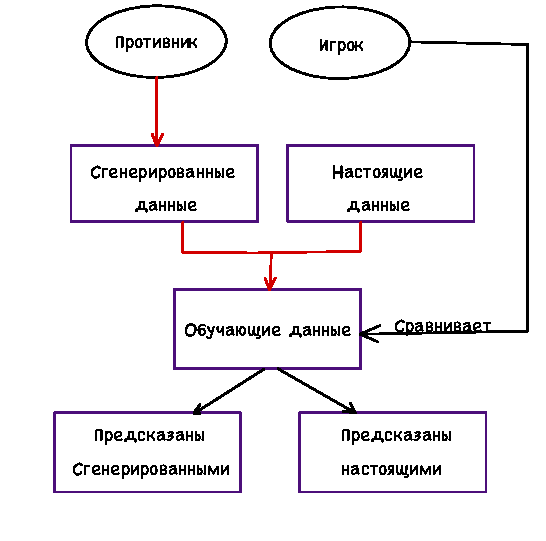
\includegraphics[width=6cm]{self-play.pdf}
            \end{figure}
        \end{column}
    \end{columns}

    
\end{frame}



%----------------------------------------------------------------------------------------------------------
\begin{frame}{Задача дообучения на этапе SFT}
    Множество $\bTheta$ - пространство всевозможных параметров, $p_{\btheta}$ - модель , а $\btheta \in \bTheta$ -  ее параметры. $\bx = [x_1, ..., x_n]\sim q(\cdot)$, $\by=[y_1, ..., y_m]\sim p_{data}(\cdot|\bx)$ - последовательности символов, интерпретируются как промпт и истинный ответ

\bigskip

В задаче ставится ограничение на количество параметров модели, то есть $\|\bTheta\| \le \mathbf{K}$

\bigskip

Модель в виде условной плотности:

$$p_{\btheta}(\by|\bx) = \prod_{j=1}^m p_{\btheta}(y_j|\bx, y_{<j})$$

Задача минимизации функционала:

\begin{align}
    L_{SFT}(\btheta) = -\EE_{\bx \sim q(\cdot), \by \sim p_{data}(\cdot|\bx)}[log p_{\btheta}(\by|\bx)]
\end{align}

\end{frame}
%----------------------------------------------------------------------------------------------------------
\begin{frame}{Двухшаговый SPIN}

\bigskip

Рассмотрим итерацию t+1, противником является $p_{\btheta_t}$, которая по промптам $\bx$ генерирует ответы $\by'$, а игроком $p_{\btheta_{t+1}}$.

\bigskip


\begin{columns}[T]
\column{0.5\textwidth}
\textcolor{blue}{Обучение игрока:}

\begin{gather*}
    \begin{align*}
        f_{t+1} &= \argmin_{f \in \cF_{t}}\EE\big[l(f(\bx, \by) - f(\bx, \by')) \big]
    \end{align*} \\
    \bx \sim q(\cdot) \\
    \by \sim p_{data}(\cdot| \bx) \\
    l(t) = log(1 + e^{-t})
\end{gather*}


    

\column{0.5\textwidth}
\textcolor{blue}{Обновление противника:}   
\begin{gather*}
  \begin{align*}
    p_{\btheta_{t+1}} = \argmax_ {p}\EE [f_{t+1}(\bx, \by)] -\\ \lambda \EE_{\bx\sim q(\cdot)}\mathrm{KL}\big(p(\cdot|\bx)||p_{\btheta_t}(\cdot|\bx)\big)
\end{align*} \\
  \bx \sim q(\cdot) \\
    \by \sim p_{data}(\cdot| \bx) \\
    l(t) = log(1 + e^{-t})
\end{gather*}
\end{columns}

\end{frame}
%----------------------------------------------------------------------------------------------------------
\begin{frame}{Одношаговый SPIN }

\bigskip

Обозначим за $\bOmega \subset \bTheta$ - подпространство весов адаптеров LoRA, малоранговых разложений обучаемых матриц

\bigskip

\textcolor{blue}{Предложенный метод}:
\begin{gather*}
 L_{SPIN}= \EE_{\bx\sim q(\cdot), \by\sim p_{data}(\cdot | \bx)}\bigg[\ell\bigg(\lambda \log \frac{p_{\btheta}(\by | \bx)}{p_{\btheta_t}(\by | \bx)}-\lambda \log \frac{p_{\btheta}(\by' | \bx)}{p_{\btheta_t}(\by' | \bx)}\bigg)\bigg]
\end{gather*}

\begin{gather*}
    \bDelta\btheta_{t+1} = \argmin_{\bDelta\btheta \in \bOmega} L_{SPIN} (\btheta_0 + \bDelta\btheta, \btheta_0 + \bDelta \btheta_t)
\end{gather*}

\end{frame}
%----------------------------------------------------------------------------------------------------------
\begin{frame}{Вычислительный эксперимент}
\begin{block}{Гипотеза}
Значения метрики у модели, обученной предложенным методом будет выше, чем у модели на этапе SFT и не будет сильно отставать от модели обученной методом SPIN
\end{block}

\begin{block}{Цель}
Обучение моделей и сравнение их по метрикам, видеопамяти и времени обучения
\end{block}

\begin{block}{Данные}
Рассматривается датасет ultrachat\_200k, модели обучаются на 1\% данных, примерно 2000 объектов
\end{block}

\end{frame}

%------------------------------------------------------------------------------------

\begin{frame}{Сравнение итераций SPIN}

\begingroup
    \fontsize{7pt}{12pt}\selectfont
   \begin{tabular}{l|l|l|l|}
        model                  & trainable params & BLEU (SFT)       & BLEU (LoRA + SPIN) \\ \hline
        qwen2.5 (lora\_r = 8)  & 1M               & 0.06454 (93.4\%) & 0.06554 (93.2\%)   \\ \hline
        qwen2.5 (lora\_r = 16) & 2.2M             & 0.06420 (92.9\%) & 0.06895 (98.0\%)   \\ \hline
        qwen2.5 (without lora) & 494M             & 0.06912 (100\%)  & 0.07035 (100\%)    \\ \hline
    \end{tabular}
    \begin{center}
        \tiny \text{Обучение моделей Qwen2.5-0.5B-Instruct. lora\_r - параметр промежуточной размерности} \\ \text{ адаптеров. Модели с адаптерами обучались на T4 (16GB), а модель без параметров на A100 (40GB)}
    \end{center}
\endgroup

\bigskip

\begin{enumerate}
  \item Снижение затрачиваемой видеопамяти в 2 раза

  \item Разница метрики модели без адаптеров с моделью с адаптерами 2%

  \item Время обучения моделей с адаптерами ~ 8-9 часов, а обучение модели без адаптеров на A100 2.5 часа
\end{enumerate}
\end{frame}
%----------------------------------------------------------------------------------------------------------
\begin{frame}{Выносится на защиту}
  \begin{enumerate}
      \item Предложен метод дообучения в услових ограниченных ресурсов
      \item Исследована оправданность применимости метода. Метод смог уменьшить используемую видеопамять в 2 раза при снижении значения метрики на 2\%
  \end{enumerate}
\end{frame}
%----------------------------------------------------------------------------------------------------------

\begin{frame}{Литература}
\begin{enumerate}
    \item
      \textcolor{black}{Zixiang Chen и др. . }
      \textcolor{blue}{«Self-Play Fine-Tuning Converts Weak Language Models to Strong Language Models»}.
    \BibJournal{Openreview},2024
	  URL: \BibUrl{https://openreview.net/forum?id=O4cHTxW9BS.}.

  \item
    \textcolor{black}{Edward J Hu и др.}
    \textcolor{blue} {LoRA: Low-Rank Adaptation of Large Language Models}
    \BibJournal{Openreview}, 2022
	  URL: \BibUrl{https://openreview.net/forum?id=nZeVKeeFYf9}.

  \item
    \textcolor{black}{Rafael Rafailov и др.}
    \textcolor{blue}{Direct Preference Optimization: Your Language Model is Secretly a Reward Model}//
    \BibJournal{NeurIps}, 2023
    
    \end{enumerate}
\end{frame}


%----------------------------------------------------------------------------------------------------------

\end{document} 